%!TEX root = paper.tex
%%%%%%%%%%%%%%%%%%%%%%%%%%%%%%%%%%%%%%%%%%%%%%%%%%%%%%%%%%%%%%%%%%%%%%%%%%%%%%%%
\section{An End-to-End Lag Model}
\label{sec:model}

%The proposed abstract lag model can be adapted to any gaming use case, be it either local, networked, or cloud games. Depending on the specific scenario, more or less components have to be factored in (e.g., the network path and game server with its discrete game ticks for an online game, or the video encoding and decoding elements in cloud gaming). Generally, it derives the \gls{E2E} lag from those factors, specifically including the framerate, tickrate, network \gls{QoS}, client/server messaging rates, and I/O characteristics. The \gls{E2E} lag is here defined to be the time elapsed between the player supplying commands to the input devices and the corresponding audio/video output. Figure~\ref{fig:queuing-model} depicts the overall queuing model.

We define the \gls{E2E} lag $T$ to be the time elapsed from when the player supplies commands to the input devices until the results of this command are displayed. We assume the player input to be a stochastic process $U$. Furthermore, input events are queued up and sent en bloc at specific intervals defined by the command rate $c$. Second, the online game variant focuses solely on modeling a single connected client and its interaction with the game server. Next, a fixed tickrate $g$ is associated with the computation process of the game server, and a framerate $f$ with the render process. The server updates the state of the game world at every tick, and may spend some processing time $P$ in order to do so. The processing time is a random variable which is assumed to follow a truncated normal distribution in our simulations. Once finished, an update message is sent to the client. Since the client needs time to render this update, it is displayed only after the next, upcoming frame. Independent of the update process, the game client outputs the next video frame in accordance to the framerate.
%The round-trip to the server and back implies that the lag between an input event and the earliest frame containing a perceptible result of that event can take multiple frame times.
While the command, tick, and framerates to be constant (though not necessarily identical), there is no inherent synchronization between them. This is represented in the simulation by a random initial phase offset for each rate.

\begin{figure}[!t]
	\centering
	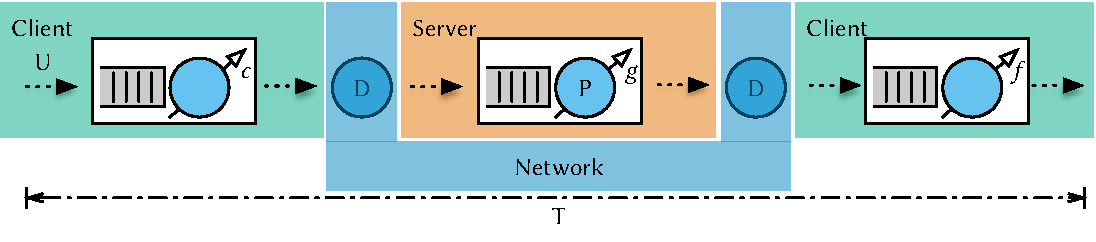
\includegraphics[width=1.0\columnwidth]{../../../models/e2e-lag-model.pdf}
	\caption{Queuing lag model in an online video game case.}
\label{fig:queuing-model}
\end{figure}


% \begin{table}[!t]
% \caption{Notation used in the model. Random variables are denoted by capital letters $X$, and constants by small letters $x$.}
% \label{tab:notation}
% 	\centering
% 	\begin{tabu}{lX[1,l]X[1,l]}
% 	\toprule
% 	\textbf{Symbol} & \textbf{Description} & \textbf{Simulation} \\
% 	\midrule
% 	$D$ & network delay between game client and server & $D \sim TNorm(\mu_D;\sigma_D)$, $\mu_D = \SI{20}{\milli\second}$; $\sigma_D = \SI{5}{\milli\second}$\\
% 	$P$ & game server processing time & $P \sim TNorm(\mu_P;\sigma_P)$, $ \mu_P = \SI{3}{\milli\second}; \sigma_P = \SI{0.1}{\milli\second}$\\
% 	$T$ & end-to-end lag & key performance measure \\
% 	$U$ & (inter arrival) time between user inputs & $U \sim Exp(\lambda)$; $\lambda = \SI{50}{\milli\second}$\\
% 	\midrule
% 	$c$ & command rate & $c=g$ \\
% 	$c^{-1}$ & interval to gather input events before sending & \\
% 	$d$ & decode delay & \SI{5}{\milli\second} \\
% 	$e$ & encode delay & \SI{15}{\milli\second} \\
% 	$f$ & framerate & $f \in \SIrange{10}{200}{\hertz}$ \\
% 	$f^{-1}$ & frame duration & $f^{-1} \in \SIrange{5}{100}{\milli\second}$ \\
% 	$g$ & game tickrate & $g \in \SIrange{10}{200}{\hertz}$ \\
% 	$g^{-1}$ & game tick duration & $g^{-1} \in \SIrange{5}{100}{\milli\second}$ \\
% 	\bottomrule
% 	\end{tabu}
% \end{table}

% \begin{figure}[!t]
% 	\centering
% 	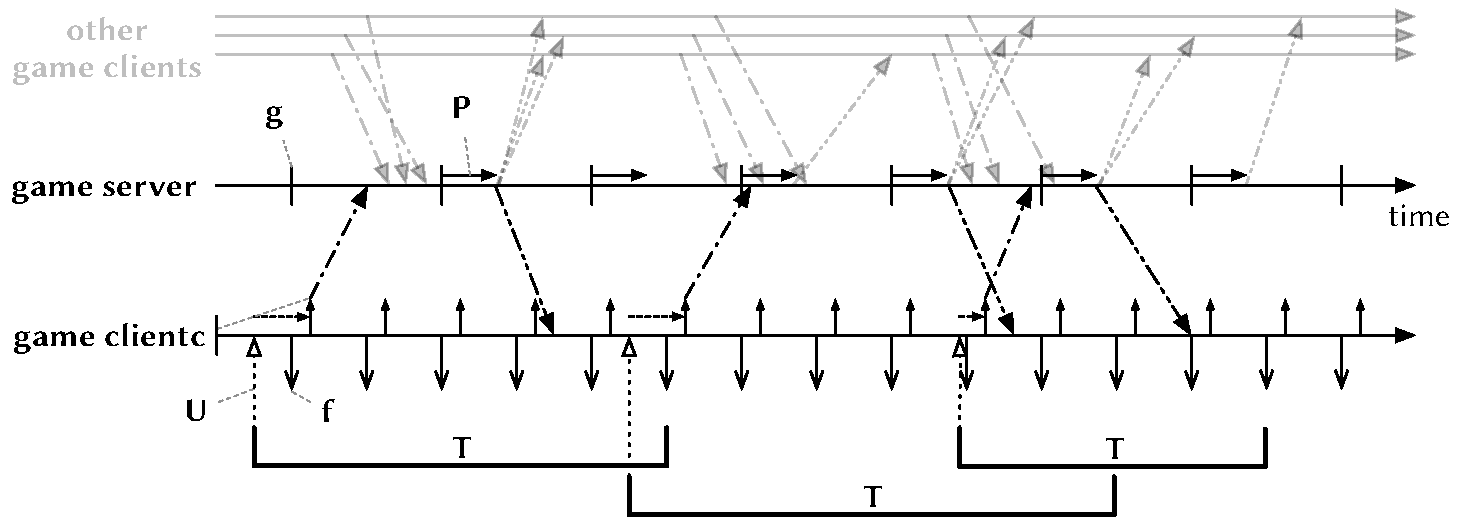
\includegraphics[width=1.0\columnwidth]{../../../models/tickrate-timeseries-notation.pdf}
% 	\caption{Exemplary flow of events in an online client-server game, and resulting end-to-end lag with the notation of Tab.~\ref{tab:notation}.
% 	% \hoss{Notation aus Tabelle ~\ref{tab:notation} waere gut im Bild. }
% 	} %Delay values are given for a framerate of \SI{60}{\hertz} and a server tickrate of \SI{30}{\hertz}, the network latency will only show minor variations.}
% \label{fig:tickrate-timeseries}
% \end{figure}

Finally, since we are simulating online games, the simulation obviously includes the network paths between the different components. The delay distributions are freely configurable, but may be omitted entirely as well. We assume a random variable $D$ representing the networking delay between game client and server. Fig.~\ref{fig:queuing-model} gives a graphical representation of the queuing model for the online video game case, especially including the three clocked processes responsible for the game's interactions. 
%Moreover, Fig.~\ref{fig:tickrate-timeseries} shows the flow of events between game client and server for the simplified case of an online video game.
The model variant for cloud gaming is based on the online game model, adapting its notions of $D$, $P$, $T$, $U$, $c$, and $f$. However, the server now handles only one client, and becomes a \textit{streaming server} that also renders and encodes the screen contents, adding a constant encoding delay $e$. On the client side, the stream is decoded (adding decoding delay $d$) before being displayed.



\subsection{Model Limitations}

These simulation models do not attempt to capture all possible sources of lag that. Indeed, we simplify the models in the following aspects in the hope to make the results more tractable. The models ignore the delays contributed by input devices like keyboards, mice, and game controllers. We estimate these at below \SI{10}{\milli\second}. The same goes for the lag of the display device (from after rendering or decoding until the frame is actually visible) which is typically in the range of $1-3$ frame times for a computer monitor, and larger for TV sets. The models can be extended to take those delay factors into account, but they were exempted for the sake of simplicity in this paper. Modern games go great lengths to handle lag gracefully, and try to ``work around it'' in various ways. The methods for this vary, and implementations usually are not open for examination, so we leave them for further study. Techniques include lag compensation (the game client tries to predict the server state from past knowledge, allowing for smoother local updates but possibly causing slight deviation and re-synchronization artifacts), and tick- and framerate adaptation at the game server and client, respectively. Lastly, player actions in a game might take multiple command time intervals to perform. The simulation currently assumes that every single batch of commands that reaches the server will result in state updates and thus changes in the perceptible output of the game client. It should be noted that none of these techniques alter the end-to-end lag itself, rather they just try to conceal it on some higher level. Therefore, the mechanisms do not invalidate our examination.

% \textbf{Factors in human perception and strategy}

% The models we present do not take into account the perceived lag from when the players \textit{think} they have triggered an action to when they perceive the outcomes of their action. This consequently disregards effects of different player actions, strategies, and so on.

